\documentclass[12pt]{article}
\usepackage[utf8]{inputenc}
\usepackage[russian]{babel}
\usepackage{titlesec}
\usepackage{titling}
\usepackage{graphicx}
\usepackage[russian]{babel}
\usepackage[babel = true]{microtype}
\usepackage[left=10mm,right=10mm, top=15mm,bottom=15mm]{geometry}
\usepackage{amsmath}
\usepackage{mathtools}
\usepackage{array}
\usepackage{wrapfig}
\usepackage{multirow}
\usepackage{tabu}
\let\oldAA\AA
\renewcommand{\AA}{\text{\normalfont\oldAA}}


\setlength{\droptitle}{-5em}

\title{Работа 4.3.4. Метод преобразования Фурье в оптике}
\date{}

\titleformat{\section}[hang]
{\normalfont\bfseries}
{\thesection.}{0.5em}{}

\titleformat{\subsection}[hang]
{\normalfont\bfseries}
{\thesection.}{0.5em}{}

\begin{document}

\maketitle

\paragraph{Цель работы:}исследование особенностей применения пространственного преобразования Фурье для анализа дифракционных явлений.

\paragraph{В работе используются:}гелий-неоновый лазер, кассета с набором сеток разного периода, щель с микрометрическим винтом, линзы, экран, линейка.

\section*{Теоретическая часть}
\begin{enumerate}
    \item Принцип Гюйгенса-Френеля:
    \[ g(x,y) = \frac{1}{i \lambda} \iint\limits_S f_0(\xi,\eta ) \frac{e^{ikR}}{R}\cos{\alpha} \,d\xi d\eta  \] 
    
    \item Дифракция Фраунгофера и преобразование Фурье. Двумерное преобразование Фурье:
    \[ g(x,y) = \frac{e^{ikR_0}}{i \lambda R_0} \iint\limits_S f_0(\xi,\eta ) e^{-i(u\xi + v\eta)} \cos{\alpha} \,d\xi d\eta,\  \text{где:} u = \frac{kx}{R_0},\ v = \frac{ky}{R_0}  \] 
    
    \item Принципы Фурье-оптики:
    \[ f(x,z) = a e^{i(k_x x+k_z z + \varphi)} = c e^{i(ux + \sqrt{k^2 - u^2} z )},\ \text{где: } k_x = u,\ c = a e^{i \varphi}  \] 
    \[ f(x,0) = c e^{iux},\ f(x,z) = f(x,0) e^{i \sqrt{k^2-u^2}z } \]
    \item Распространение волн:
    \[ f(x,z)= \int C_0(u) e^{i(ux+\sqrt{k^2-x^2}z) } \,du\ \text{где: }C_0(u) \text{ --- преобразование Фурье граничного поля} \]
    \item Передаточная функция:
    \[ H(u) = e^{i\sqrt{k^2-x^2}z} \]
    
\end{enumerate}


\section*{Экспериментальная установка:}
\begin{enumerate}
    
\begin{figure}[h!]
    \noindent\centering{
        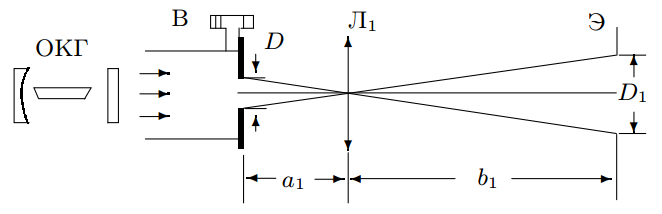
\includegraphics[height = 4cm]{Selection_024.png}
    }
    \caption{Схема для определения ширины щели с помощью линзы}
\end{figure}

\item Ширину щели будем определять, используя формулу для увеличения изображения:

\begin{equation}
\label{1}
    \Gamma = \frac{D_1}{D} = \frac{b_1}{a_1}
\end{equation}  

\begin{figure}[h!]
    \noindent\centering{
        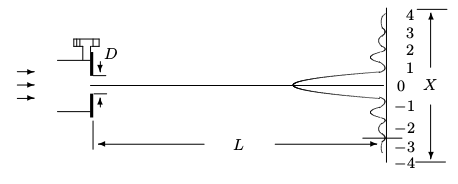
\includegraphics[height = 4cm]{Selection_026.png}
    }
    \caption{Схема для определения ширины щели по спектру}
\end{figure}

\item  Для определения ширины щели по спекту $b_c$ будем использовать соотношение:

\begin{equation}
\label{2}
    \Delta X = \frac{X}{2m} = \frac{\lambda}{b_c}L
\end{equation}  

\begin{figure}[h!]
    \noindent\centering{
        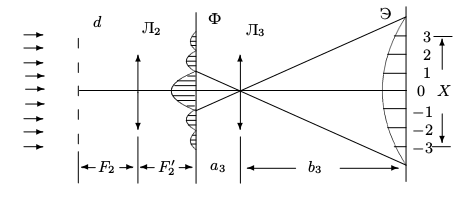
\includegraphics[height = 4cm]{Selection_027.png}
    }
    \caption{Схема определения периода решётки по
увеличенному изображению спектра}
\end{figure}

\item Для определния периода решеток нам понадобится расстояние $X$ между $m$-ми максимумами. Тогда:

\begin{equation}
\label{3}
    \Delta X = \frac{X}{2m} = \frac{\lambda}{d_c}L
\end{equation}  

\item В этом эксперименте можно рассчитать расстояние между соседними максимумами $\Delta x$ в плоскости $\Phi$ и период сетки $d$ используя формулу:

\begin{equation}
\label{4}
    \Delta x = \frac{\Delta X}{\Gamma_3} = \frac{\lambda}{d_l}F_2
\end{equation}  


\begin{figure}[h!]
    \noindent\centering{
        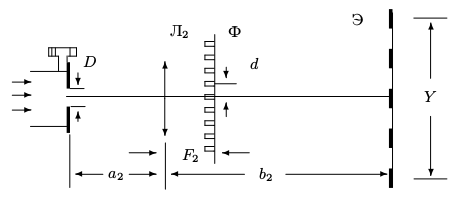
\includegraphics[height = 4cm]{Selection_028.png}
    }
    \caption{Схема для наблюдения мультиплицирования}
\end{figure}

\item Периоды "фиктивных" решеток связаны с периодом решеток, определенных по спектру, связаны следующей формулой:


\begin{equation}
\label{5}
    \frac{\lambda}{\Delta y} F_2 = d_c 
\end{equation} 

\end{enumerate}

\newpage

\section*{Ход работы}

\subsection*{А. Определение  ширины щели}

\paragraph{I. Определение ширины щели по увеличенному изображению}
\begin{enumerate}
    \item С помощью короткофокусной линзы $ L_1 $ ($ F_1 = 38\text{mm} $) получаем на экране изображение щели
    
    \item Определим начало отсчета ширины щели по ее открытию --- $D_0 = -30 \mu \text{m} $    
    
    \item Меняя ширину щели будем снимать зависимость размеров изображения $ D_1 $ от ширины щели $b$. Сведем измерения в таблицу:\\
    \begin{tabu} to 1.2\textwidth{|c|c|c|c|c|c|c|c|c|c|}
    \hline
    Ширина щели $\tilde D, \mu m$ & 20 & 70 & 120 & 170 & 220 & 270 & 320 & 370 & 420 \\
    \hline
    $\tilde D + D_0, \mu m$ & 50 & 100 & 150 & 200 & 250 & 300 & 350 & 400 & 450 \\
    \hline
    Размер изображения $D_1$, $mm$ & 1.5 & 3 & 4 & 5 & 7 & 8 & 9 & 11 & 12 \\
    \hline
    \end{tabu}
    
    \item Измерим расстояния $a_1$, $b_1$ и $L$ для рассчета увеличения системы $\Gamma$ по формуле \ref{1}:\\
    $a_1 = 4 \pm 0.1 cm,\\  b_1 = 134 \pm 0.5 cm,\\ L = 139 \pm 0.5 cm $
    \begin{equation}
        \Gamma = \frac{b_1}{a_1} = \frac{134 cm}{4 cm} = 33.5 \pm 0.9 
    \end{equation}  
    
    \item Зная увеличение линзы и размер изображения, рассчитаем по формуле \ref{1} ширину щели $D'$. Резульаьты сведем в таблицу: \\
    \begin{tabu} to 1\textwidth{|c|c|c|c|c|c|c|c|c|c|}
    \hline
    Размер изображения $D_1$, $mm$ & 1.5 & 3 & 4 & 5 & 7 & 8 & 9 & 11 & 12 \\
    \hline
    Рассчитанная ширина $D'$, $\mu m$ & 45 & 89 & 149 & 208 & 238 & 268 & 327 & 387 & 446 \\
    \hline
    Погрешность & 1.7 & 3.8 & 4.7 & 5.3 & 7.8 & 8.3 & 9.5 & 11.6 & 12.7\\
    \hline
    Ширина щели $D$, $\mu m$ & 50 & 100 & 150 & 200 & 250 & 300 & 350 & 400 & 450 \\
    \hline
    Относительная погрешность, \% & 10.8 & 10.6 & 0.9 & 4.1 & 4.8 & 10.3 & 6.5 & 3.4 & 0.9\\
    \hline
    \end{tabu}

\end{enumerate}

\paragraph{II. Определение ширины щели по её спектру}
\begin{enumerate}
    \item На удаленном экране получим спектр шели. Оценим отнервал, в котором можно наблюдать и измерять спектр: \\
    \[ D \in [ 0\mu m - 45\mu m ] \]
    
    \item Измерим ширину спектра для щелей разной ширины. Рассчитаем ширину щели, используя формулу \ref{2}, используя значение длинны волны He-Ne-лазера $ \lambda = 6328 \AA $. Результаты сведем в таблицу:\\
    \begin{tabu} to 1\textwidth{|c|c|c|c|c|c|c|c|c|c|}
    \hline
    Ширина щели $D$, $\mu m$ & 50 & 100 & 150 & 200 & 250 & 300 & 350 & 400 \\
    \hline
    Расстояние $\Delta X$ & 35 & 20 & 13 & 8 & 6 & 5 & 4 & 3 \\
    \hline
    Ширина щели $b_s$, $\mu m$ & 42 & 74 & 113 & 184 & 246 & 294 & 368 & 431 \\
    \hline
    Погрешность & 15.7 & 26.3 & 24.4 & 7.8 & 1.7 & 1.8 & 5.3 & 22 \\
    \hline
    \end{tabu}
    
    \item На одном графике построим зависимости $ b_l = f(b)\ \text{и}\ b_s = f(b) $:
    \begin{figure}[h!]
    \noindent\centering{
        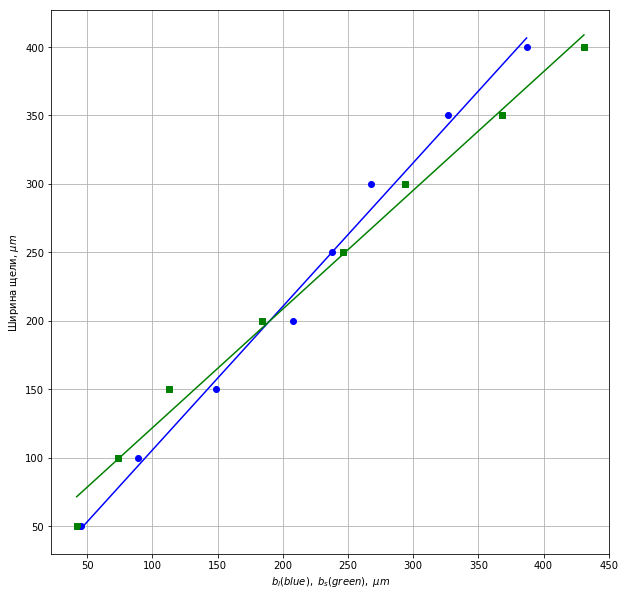
\includegraphics[height = 10cm]{download1.png}
    }
    \caption{Сравнение результатов первого и второго экспериментов}
\end{figure}
    
\end{enumerate}

\newpage

\subsection*{Б. Определение периода решёток}

\paragraph{III. Определение периода по спектру на удалённом экране}
\begin{enumerate}
    \item Bычислим расстояние $L$. К выходу лазера поставим кассету с двумерными решетками. Для каждой сетки измерим расстояние $X$ между $m$-ми максимумами и рассчитаем $\Delta X$ и период каждой решетки $d_c$ по формуле \ref{3}. Результаты сведем в табилцу: \\
    $L = 138.5 cm$ \\
    \begin{tabu} to 1\textwidth{|c|c|c|c|c|c|}
    \hline
    Решетка $№$ & 1 & 2 & 3 & 4 &  6 \\
    \hline
    Расстояние $X, mm$ & 44 & 37 & 92 & 73 & 80 \\
    \hline
    Порядок минимума $m$ & 10 & 1 & 5 & 5 & 10 \\
    \hline
    $\Delta X, mm$ & 4.4 & 37 & 18.4 & 14.6 & 8 \\
    \hline
    $d_c, \mu m$ & 334 & 39 & 80 & 101 & 184 \\
    \hline
    \end{tabu}
        
\end{enumerate}
    
\paragraph{IV. Определение периода решёток по увеличенному изображению спектра}
\begin{enumerate}
    \item Установим линзу с максимальным фокусным расстоянием ($F_2 = 110 mm$ ) на расстоянии примерно равном фокусному от кассеты. В плоскости $\Phi$ мы получиил фурье-образ сетки, а которкофокусная линза ($F_3 = 23 mm$ ) создает на экране увеличенное изображение этого спектра.
    
    \item Рассчитаем увеличение короткофокусной линзы: \\
    $ a_3 = 2.8 \pm 0.1 cm $ \\ 
    $ b_3 = 110.5 \pm 0.5 cm  $ \\
    \[ \Gamma = \frac{b_3}{a_3} = \frac{110.5 cm}{2.8 cm} = 39.5 \pm 1.1 \]
    
    \item Измерим $X$ и $m$ для всех сеток, где это возможно. Теперь по формуле \ref{4} рассчитаем расстояние между максимумами $\Delta x$ и период сетки $d_l$. Результаты сведем в таблицу: \\
    \begin{tabu} to 1\textwidth{|c|c|c|c|c|c|c|}
    \hline
    Решетка $№$ & 1 & 2 & 3 & 4 & 5 & 6 \\
    \hline
    Расстояние $X, mm$ & 65 & 103 & 105 & 125 & 126 & 102 \\
    \hline
    Порядок минимума $m$ & 5 & 1 & 2 & 3 & 3 & 5 \\
    \hline
    $ \Delta X, mm $ & 13 & 103 & 52.5 & 41.7 & 42 & 20.4 \\
    \hline
    $ d_l, \mu m $ & 355 & 45 & 88 & 110 & 111 & 226 \\
    \hline
    \end{tabu}
    
\end{enumerate}

\subsection*{В. Пространственное преобразование спектров}

\paragraph{V. Мультиплицирование}
\begin{enumerate}
    \item С помощью линзы с максимальным фокусом получим в резкое изображение щели. В фокальной плоскости линзы установим кассету с сетками, которые будут осуществлять пространственную фильтрацию. 
    \item Подберем такую ширину входной щели $D$, чтобы на экране можно было наблюдать мультиплицированное изображение для любой сетки. Рассчиаем увеличение линзы. \\
    $ D = 140 \mu m $ \\
    $ F_2 =  110 mm $ \\
    $ a_2 = 10.5 \pm 0.1 cm $ \\
    $ b_2 = 127 \pm 0.5 cm $ \\
    \[ \Gamma_2 = \frac{b_2}{a_2} = \frac{127 cm}{10.5 cm} = 12.1 \pm 0.2 \]
    \item Снимем зависимость $Y$(расстояния между удаленными изображенями щели) и $K$(число промежутков между изображениями) для каждой из сеток. По полученным данным рассчитаем периоды $\Delta y :\ \Delta y = \Delta Y / \Gamma_2, \text{ где: } \Delta Y = Y/K$. Запишем результаты: \\
    \begin{tabu} to 1\textwidth{|c|c|c|c|c|c|c|}
    \hline
    Решетка $№$ & 1 & 2 & 3 & 4 & 5 & 6 \\
    \hline
    Расстояние $Y, mm$ & 18 & 90 & 75 & 60 & 72 & 30 \\
    \hline
    $K$ & 5 & 3 & 5 & 5 & 6 & 5 \\
    \hline
    $ \Delta Y, mm $ & 3.6 & 30 & 15 & 12 & 12 & 6 \\
    \hline
    $ \Delta y, mm $ & 2.9 & 24.8 & 12.4 & 9.9 & 9.9 & 5.0 \\
    \hline
    \end{tabu}
    
    
    \item Построим график $\Delta y = f(1/d_c)$:
    \begin{figure}[h!]
    \noindent\centering{
        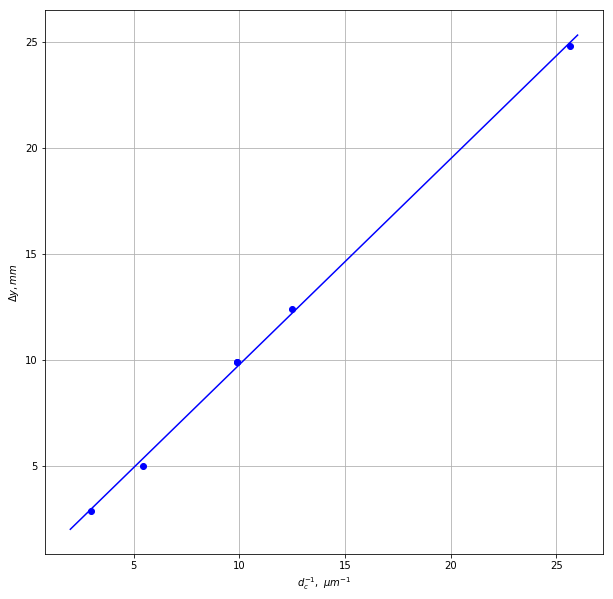
\includegraphics[height = 10cm]{download2.png}
    }
    \caption{Зависимость $\Delta y(1/d_c)$}
\end{figure}
    
\end{enumerate}

\newpage
%\paragraph{VI. Влияние щелевой диафрагмы на изображение сетки
%(пространственная фильтрация)}

\paragraph{Вывод:} исследовали особенности применения пространственного преобразования Фурье для анализа дифракционных явлений.

\end{document}
